\documentclass[11pt,a4paper]{article}
\usepackage[margin=1in]{geometry}
\usepackage{amsmath,amssymb}
\usepackage{booktabs}
\usepackage{graphicx}
\usepackage{hyperref}
\usepackage[numbers]{natbib}
\usepackage{xcolor}
\usepackage{siunitx}
\sisetup{group-separator={,}, group-minimum-digits=4}
\usepackage{tikz}
\usetikzlibrary{arrows.meta,positioning,shapes.geometric}
\usepackage{float}
\usepackage{enumitem}
\usepackage{caption}
\usepackage{longtable}

\hypersetup{
    colorlinks=true,
    linkcolor=blue!70!black,
    citecolor=green!50!black,
    urlcolor=cyan!60!black,
}

\title{Techno-Economic Assessment of\\[4pt] \textbf{Steel Slag} Valorization\\[6pt]
\large H\textsubscript{2} Production, CO\textsubscript{2} Sequestration, and Iron Recovery}
\author{Step Function LLC\\[2pt] \small Separation-Agents Framework}
\date{\today}

\begin{document}

\maketitle

\begin{abstract}
This study presents a techno-economic assessment of valorizing basic oxygen furnace (BOF)
steel slag through three integrated pathways: hydrogen production via serpentinization,
CO\textsubscript{2} sequestration via mineral carbonation, and iron concentrate recovery via
magnetic separation.  A Generalized Disjunctive Programming (GDP) superstructure with 4
feasible topologies was evaluated at \SI{500}{t/d} throughput using the Separation-Agents
framework.  Reaktoro thermodynamic speciation informed the equilibrium constraints, and
JAX-based techno-economic analysis (TEA) ranked all configurations.  The optimal topology
(heat recovery only, no inter-reactor scrubber) yields a net value of
\textbf{\$\num{37.87}/t} feedstock (\$\num{6.25}M/yr), driven by iron concentrate revenue
(\$\num{5.05}M/yr), CO\textsubscript{2} credits (\$\num{3.51}M/yr), and green hydrogen
(\$\num{0.96}M/yr).
\end{abstract}

\tableofcontents
\clearpage

%% ═══════════════════════════════════════════════════════════════════
\section{Introduction and Opportunity}
%% ═══════════════════════════════════════════════════════════════════

Basic oxygen furnace (BOF) steel slag is a high-volume industrial byproduct generated at
rates of 100--200\,kg per tonne of crude steel.  Global steel production exceeds
\SI{1.8e9}{t/yr}, yielding over \SI{250e6}{t/yr} of BOF slag~\cite{worldsteel2023}.
While some slag is recycled as construction aggregate, the majority is landfilled,
representing both an environmental liability and a missed resource opportunity.

BOF slag's mineral composition---rich in CaO, FeO/Fe\textsubscript{2}O\textsubscript{3},
MgO, and SiO\textsubscript{2}---makes it an attractive feedstock for:
\begin{enumerate}[nosep]
    \item \textbf{Green hydrogen} via serpentinization of fayalite
          (Fe\textsubscript{2}SiO\textsubscript{4}),
    \item \textbf{CO\textsubscript{2} sequestration} via mineral carbonation of CaO and MgO, and
    \item \textbf{Iron concentrate recovery} via low-intensity magnetic separation (LIMS).
\end{enumerate}

This study applies the Separation-Agents GDP optimization framework to identify the
process topology that maximizes net economic value per tonne of slag.

%% ═══════════════════════════════════════════════════════════════════
\section{Raw Material Composition}
%% ═══════════════════════════════════════════════════════════════════

The BOF steel slag composition assumed in this study is representative of typical
converter slag from integrated steelworks.

\begin{table}[H]
\centering
\caption{BOF steel slag composition (wt\%).}
\label{tab:composition}
\begin{tabular}{@{}lcc@{}}
\toprule
\textbf{Component} & \textbf{wt\%} & \textbf{Role in Valorization} \\
\midrule
CaO                & 40 & CO\textsubscript{2} mineralization $\to$ CaCO\textsubscript{3} \\
Fe\textsubscript{2}O\textsubscript{3} & 15 & Iron concentrate; oxide feed \\
FeO                & 15 & Fayalite source for H\textsubscript{2}; iron recovery \\
SiO\textsubscript{2} & 20 & Gangue (reports to quartz) \\
MgO                & 10 & CO\textsubscript{2} mineralization $\to$ MgCO\textsubscript{3} \\
\bottomrule
\end{tabular}
\end{table}

%% ═══════════════════════════════════════════════════════════════════
\section{Process Description}
%% ═══════════════════════════════════════════════════════════════════

The process comprises three sequential stages, informed by Reaktoro
equilibrium speciation results showing that iron removal is required
before carbonation to maintain a pH favorable for carbonate precipitation.

\subsection{Process Flow Diagram}

\begin{figure}[H]
\centering
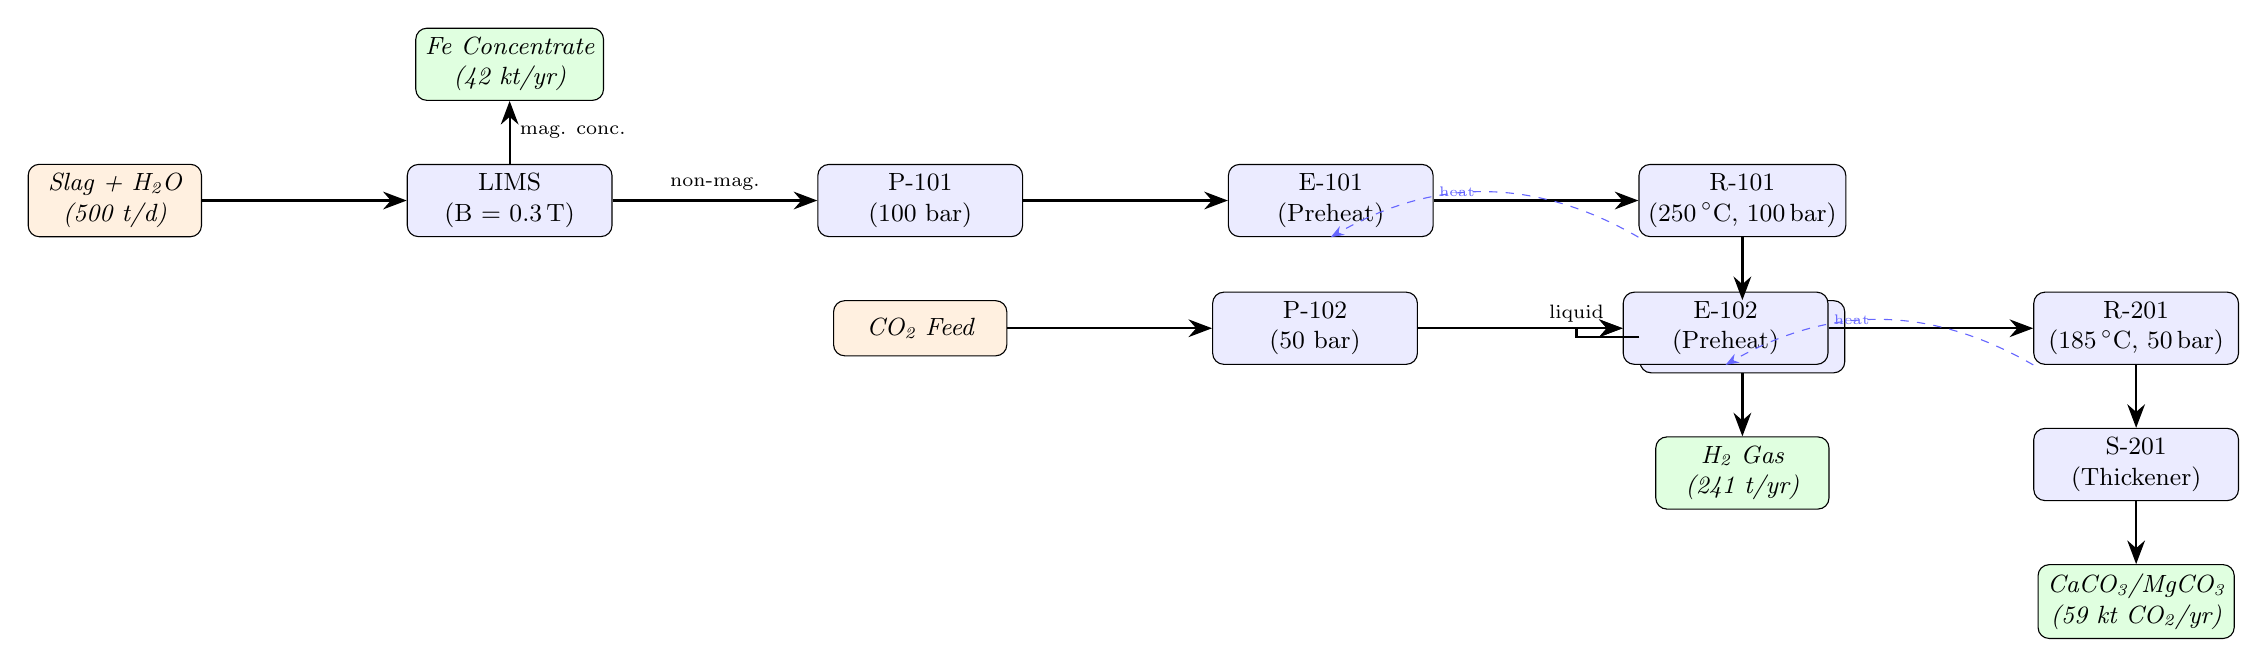
\begin{tikzpicture}[
  node distance=1.6cm and 2.6cm,
  unit/.style={rectangle, draw, rounded corners=4pt, minimum width=2.6cm,
               minimum height=0.9cm, align=center, fill=blue!8, font=\small},
  product/.style={rectangle, draw, rounded corners=4pt, minimum width=2.2cm,
                  minimum height=0.7cm, align=center, fill=green!12,
                  font=\small\itshape},
  feed/.style={rectangle, draw, rounded corners=4pt, minimum width=2.2cm,
               minimum height=0.7cm, align=center, fill=orange!12,
               font=\small\itshape},
  stream/.style={-{Stealth[length=3mm]}, thick},
]

% Feed
\node[feed] (slag) {Slag + H\textsubscript{2}O\\(500 t/d)};

% Stage 1: Magnetic separation
\node[unit, right=of slag] (lims) {LIMS\\(B = 0.3\,T)};

% Iron product
\node[product, above=0.8cm of lims] (fe) {Fe Concentrate\\(42 kt/yr)};

% Stage 2: Serpentinization
\node[unit, right=of lims] (pump) {P-101\\(100 bar)};
\node[unit, right=of pump] (hx1) {E-101\\(Preheat)};
\node[unit, right=of hx1] (serp) {R-101\\(\SI{250}{\celsius}, \SI{100}{bar})};

% H2 separation
\node[unit, below=0.8cm of serp] (sep_h2) {S-101\\(Flash Sep.)};
\node[product, below=0.8cm of sep_h2] (h2) {H\textsubscript{2} Gas\\(241 t/yr)};

% Stage 3: Carbonation
\node[feed, below=0.8cm of pump] (co2) {CO\textsubscript{2} Feed};
\node[unit, right=of co2] (pump2) {P-102\\(50 bar)};
\node[unit, right=of pump2] (hx2) {E-102\\(Preheat)};
\node[unit, right=of hx2] (carb) {R-201\\(\SI{185}{\celsius}, \SI{50}{bar})};
\node[unit, below=0.8cm of carb] (sep_c) {S-201\\(Thickener)};
\node[product, below=0.8cm of sep_c] (caco3) {CaCO\textsubscript{3}/MgCO\textsubscript{3}\\(59 kt CO\textsubscript{2}/yr)};

% Connections
\draw[stream] (slag) -- (lims);
\draw[stream] (lims) -- node[right, font=\scriptsize]{mag. conc.} (fe);
\draw[stream] (lims) -- node[above, font=\scriptsize]{non-mag.} (pump);
\draw[stream] (pump) -- (hx1);
\draw[stream] (hx1) -- (serp);
\draw[stream] (serp) -- (sep_h2);
\draw[stream] (sep_h2) -- (h2);
\draw[stream] (sep_h2.west) -- ++(-0.8,0) |- node[above, near start, font=\scriptsize]{liquid} (hx2);
\draw[stream] (co2) -- (pump2);
\draw[stream] (pump2) -- (hx2);
\draw[stream] (hx2) -- (carb);
\draw[stream] (carb) -- (sep_c);
\draw[stream] (sep_c) -- (caco3);

% Heat recovery arrows (dashed)
\draw[-{Stealth}, dashed, blue!60] (serp.south west) to[bend right=30]
    node[left, font=\tiny, blue!60]{heat} (hx1.south);
\draw[-{Stealth}, dashed, blue!60] (carb.south west) to[bend right=30]
    node[left, font=\tiny, blue!60]{heat} (hx2.south);

\end{tikzpicture}
\caption{Process flow diagram for steel slag valorization (optimal topology: heat recovery only).}
\label{fig:pfd}
\end{figure}

\subsection{Stage 1: Magnetic Separation}

Low-intensity magnetic separation (LIMS) recovers magnetite
(Fe\textsubscript{3}O\textsubscript{4}) and hematite from the slag at 85\% recovery.
The iron concentrate (approx.\ 42,000\,t/yr at 500\,t/d) is sold directly.

\subsection{Stage 2: Serpentinization — H\textsubscript{2} Production}

The non-magnetic fraction, rich in fayalite (Fe\textsubscript{2}SiO\textsubscript{4}),
undergoes serpentinization:
\begin{equation}
    \text{Fe}_2\text{SiO}_4 + 3\,\text{H}_2\text{O}
    \longrightarrow
    2\,\text{Fe(OH)}_2 + \text{SiO}_2 + \text{H}_2
    \label{eq:serp}
\end{equation}
Conditions: \SI{250}{\celsius}, \SI{100}{bar}, \SI{4}{h} residence time, 70\% conversion.
Reaktoro speciation at these conditions predicts pH~5.6 and formation of magnetite as a
secondary product.

\subsection{Stage 3: Mineral Carbonation — CO\textsubscript{2} Sequestration}

The liquid effluent from serpentinization (now depleted in iron, raising the pH)
contacts CO\textsubscript{2} at \SI{185}{\celsius} and \SI{50}{bar}:
\begin{align}
    \text{CaO} + \text{CO}_2 &\longrightarrow \text{CaCO}_3 \label{eq:carb_ca} \\
    \text{MgO} + \text{CO}_2 &\longrightarrow \text{MgCO}_3 \label{eq:carb_mg}
\end{align}
At 80--85\% conversion, approximately \SI{58575}{t} CO\textsubscript{2} per year is
permanently sequestered as stable carbonate minerals.

%% ═══════════════════════════════════════════════════════════════════
\section{Modeling Approach}
%% ═══════════════════════════════════════════════════════════════════

\begin{table}[H]
\centering
\caption{Three-tier modeling hierarchy.}
\label{tab:models}
\begin{tabular}{@{}p{3cm}p{3.5cm}p{5.5cm}@{}}
\toprule
\textbf{Tier} & \textbf{Tool} & \textbf{Role} \\
\midrule
Thermodynamic   & Reaktoro (SUPCRTBL) & Gibbs energy minimization for aqueous speciation, mineral saturation indices, pH and Eh prediction \\
Process         & IDAES-PSE + Pyomo.GDP & Sequential-modular/equation-oriented flowsheet simulation; GDP topology optimization \\
Economic        & JAX TEA & Differentiable cost modeling (CAPEX/OPEX); autodiff-based sensitivity analysis \\
\bottomrule
\end{tabular}
\end{table}

\subsection{Thermodynamic Speciation}

Three Reaktoro equilibrium scenarios were evaluated:

\begin{table}[H]
\centering
\caption{Reaktoro speciation results for steel slag.}
\label{tab:speciation}
\begin{tabular}{@{}lccp{6cm}@{}}
\toprule
\textbf{Scenario} & \textbf{pH} & \textbf{$E_h$ (V)} & \textbf{Key Finding} \\
\midrule
Ambient (25\textdegree C, 1\,atm) & 2.43 & 0.656 & Fe$^{3+}$ hydrolysis dominates; highly acidic \\
Serpentinization (250\textdegree C, 100\,bar) & 5.60 & 0.661 & 0.7\% fayalite equilibrium conversion; H$_2$(aq) produced \\
Carbonation (150\textdegree C, 50\,bar, +CO$_2$) & 3.20 & 0.106 & $<$0.1\% CO$_2$ conversion at low pH \\
\bottomrule
\end{tabular}
\end{table}

\noindent\textbf{Critical insight}: Iron removal must precede carbonation, as dissolved
Fe$^{3+}$ suppresses pH to $\sim$2--3, thermodynamically preventing carbonate precipitation.

\subsection{GDP Superstructure}

The \texttt{steel\_slag\_h2\_co2} superstructure contains 15 unit operations
(12 fixed, 3 optional) with:
\begin{itemize}[nosep]
    \item 1 disjunction: auxiliary heater \texttt{XOR} heat-recovery-only
    \item 1 optional unit: inter-reactor scrubber
    \item 4 feasible topologies
    \item 12 continuous design variables (reactor $T$, $P$, $\tau$; HX areas; pump heads)
\end{itemize}

%% ═══════════════════════════════════════════════════════════════════
\section{Cost Model Assumptions}
%% ═══════════════════════════════════════════════════════════════════

\begin{table}[H]
\centering
\caption{Plant-level parameters.}
\label{tab:plant}
\begin{tabular}{@{}lr@{}}
\toprule
\textbf{Parameter} & \textbf{Value} \\
\midrule
Slag throughput            & \SI{500}{t/d} \\
Operating days             & 330\,d/yr \\
Annual throughput          & \SI{165000}{t/yr} \\
Discount rate              & 8\% \\
Project lifetime           & 20\,yr \\
\bottomrule
\end{tabular}
\end{table}

\begin{table}[H]
\centering
\caption{Commodity prices.}
\label{tab:prices}
\begin{tabular}{@{}lrl@{}}
\toprule
\textbf{Product} & \textbf{Price} & \textbf{Source} \\
\midrule
H\textsubscript{2} (green)       & \$4/kg      & DOE target \\
CO\textsubscript{2} credit       & \$60/t      & Voluntary carbon market \\
Fe concentrate                   & \$120/t     & FOB spot \\
\bottomrule
\end{tabular}
\end{table}

%% ═══════════════════════════════════════════════════════════════════
\section{Results}
%% ═══════════════════════════════════════════════════════════════════

\subsection{Topology Ranking}

\begin{table}[H]
\centering
\caption{Trade-study results ranked by net value.}
\label{tab:tradeStudy}
\begin{tabular}{@{}clccccc@{}}
\toprule
\textbf{Rank} & \textbf{Topology} & \textbf{CAPEX} & \textbf{OPEX}
  & \textbf{EAC} & \textbf{Revenue} & \textbf{Net Value} \\
& & (\$M) & (\$M/yr) & (\$M/yr) & (\$M/yr) & (\$M/yr) \\
\midrule
1 & Heat recovery only        & 7.76 & 2.49 & 3.28 & 9.53 & \textbf{6.25} \\
2 & HR + scrubber             & 7.96 & 2.49 & 3.30 & 9.53 & 6.23 \\
3 & Aux heater                & 8.06 & 3.07 & 3.89 & 9.53 & 5.64 \\
4 & Aux heater + scrubber     & 8.26 & 3.07 & 3.91 & 9.53 & 5.62 \\
\bottomrule
\end{tabular}
\end{table}

\subsection{Revenue Breakdown}

\begin{table}[H]
\centering
\caption{Annual revenue by product stream (optimal topology).}
\label{tab:revenue}
\begin{tabular}{@{}lrrr@{}}
\toprule
\textbf{Product} & \textbf{Production} & \textbf{Price} & \textbf{Revenue (\$M/yr)} \\
\midrule
Fe concentrate  & \SI{42075}{t/yr}  & \$120/t  & 5.05 \\
CO\textsubscript{2} credits & \SI{58575}{t/yr} & \$60/t CO\textsubscript{2} & 3.51 \\
H\textsubscript{2} gas & \SI{241}{t/yr} & \$4/kg & 0.96 \\
\midrule
\textbf{Total}  & & & \textbf{9.53} \\
\bottomrule
\end{tabular}
\end{table}

\subsection{Levelized Economics}

\begin{table}[H]
\centering
\caption{Levelized economics for the optimal topology (Config 3).}
\label{tab:levelized}
\begin{tabular}{@{}lr@{}}
\toprule
\textbf{Metric} & \textbf{Value} \\
\midrule
Total CAPEX              & \$\num{7.76}M \\
Annual OPEX              & \$\num{2.49}M/yr \\
EAC (8\%, 20\,yr)        & \$\num{3.28}M/yr \\
Total Revenue            & \$\num{9.53}M/yr \\
\midrule
\textbf{Net Value}       & \textbf{\$\num{6.25}M/yr} \\
\textbf{Net Value/t}     & \textbf{\$\num{37.87}/t} \\
\bottomrule
\end{tabular}
\end{table}

\subsection{Cost Sensitivity}

JAX autodifferentiation identified the top cost drivers
($\partial$EAC/$\partial$parameter):

\begin{table}[H]
\centering
\caption{Top-5 cost sensitivity parameters (JAX autodiff).}
\label{tab:sensitivity}
\begin{tabular}{@{}lrl@{}}
\toprule
\textbf{Parameter} & \textbf{$|\partial\text{EAC}/\partial x|$} & \textbf{Interpretation} \\
\midrule
Residence time (h)       & \$\num{10185}/h  & Reactor sizing driver \\
Operating temp (\textdegree C) & \$\num{8250}/\textdegree C & Energy cost driver \\
Throughput (t/d)         & \$\num{5214}/t/d & Economies of scale \\
\bottomrule
\end{tabular}
\end{table}

%% ═══════════════════════════════════════════════════════════════════
\section{Discussion}
%% ═══════════════════════════════════════════════════════════════════

\subsection{Economic Drivers}

Iron concentrate dominates revenue at 53\% of total, followed by
CO\textsubscript{2} credits (37\%) and H\textsubscript{2} (10\%).  The marginal
value of the auxiliary heater ($-$\$\num{0.61}M/yr net) does not justify the
additional \$\num{0.30}M CAPEX and \$\num{0.58}M/yr heating OPEX.  Similarly, the
inter-reactor scrubber provides minimal benefit ($-$\$\num{0.02}M/yr).

\subsection{Key Risks}

\begin{itemize}[nosep]
    \item \textbf{CO\textsubscript{2} credit volatility}: At \$30/t (instead of \$60/t),
          CO\textsubscript{2} revenue halves to \$\num{1.76}M/yr, reducing net value
          to \$\num{4.49}M/yr (\$\num{27.22}/t).
    \item \textbf{Serpentinization kinetics}: Reaktoro predicts only 0.7\% equilibrium
          conversion in batch; achieving 70\% requires extended residence time and
          catalytic enhancement.
    \item \textbf{Iron price sensitivity}: Fe concentrate at \$80/t (vs.\ \$120/t) would
          reduce revenue by \$\num{1.68}M/yr.
\end{itemize}

\subsection{Modeling Limitations}

\begin{enumerate}[nosep]
    \item Reaktoro speciation uses the SUPCRTBL database, which lacks Cr, Mn, and V
          species commonly present in BOF slag.
    \item Serpentinization kinetics are not modeled; the 70\% conversion is assumed
          based on literature values for autoclave reactors.
    \item The JAX TEA model uses simplified cost correlations; detailed vendor quotes
          would be needed for a bankable feasibility study.
\end{enumerate}

%% ═══════════════════════════════════════════════════════════════════
\section{Conclusions}
%% ═══════════════════════════════════════════════════════════════════

\begin{enumerate}
    \item Steel slag valorization at \SI{500}{t/d} is economically attractive, yielding
          a net value of \textbf{\$\num{37.87}/t} feedstock (\$\num{6.25}M/yr).
    \item The optimal topology (heat recovery only, no scrubber) minimizes cost while
          maintaining all three revenue streams.
    \item Iron concentrate is the dominant value driver (53\% of revenue), followed by
          CO\textsubscript{2} credits (37\%) and H\textsubscript{2} (10\%).
    \item Iron removal before carbonation is thermodynamically essential (Reaktoro-confirmed).
    \item The auxiliary heater and scrubber do not justify their added cost; heat recovery
          from product streams is sufficient.
\end{enumerate}

%% ═══════════════════════════════════════════════════════════════════
\bibliographystyle{plainnat}
\begin{thebibliography}{9}

\bibitem{worldsteel2023}
World Steel Association,
\emph{Steel Statistical Yearbook 2023}.
Brussels, 2023.

\bibitem{seyfried2007}
W.~E. Seyfried et~al.,
``The effect of redox on the relative solubilities of Fe and Mn in a mid-ocean ridge
hydrothermal system,''
\emph{Geochimica et Cosmochimica Acta}, vol.~71, pp.~3724--3739, 2007.

\bibitem{leal2015}
A.~M.~M. Leal, D.~A. Kulik, and G. Kosakowski,
``Computational methods for reactive transport modeling,''
\emph{Reviews in Mineralogy and Geochemistry}, vol.~80, pp.~471--524, 2015.

\bibitem{zimmer2016}
K.~Zimmer et~al.,
``SUPCRTBL: A revised and extended thermodynamic dataset for surface and ground water
geochemistry,''
\emph{Computers \& Geosciences}, vol.~90, pp.~97--111, 2016.

\end{thebibliography}

\end{document}
